\documentclass{article}
\usepackage{graphicx}
\usepackage{listings}
\usepackage{siunitx}
\usepackage{placeins}
\usepackage{amsmath}

\begin{document}

This program generates a graph where the nodes represent different countries and the edge weights represent the "economic" influence that they have on each other. The nodes are initialized with random GDP values scaled by 100 trillion. The edge weights are based on the gdp of the country where countries with lower gdp have less economic influence than countries with a higher GDP
The weights are also dynamically updated at every time step to re-adjust for the new GDP values. 
\begin{figure}[htbp]
    \centering
    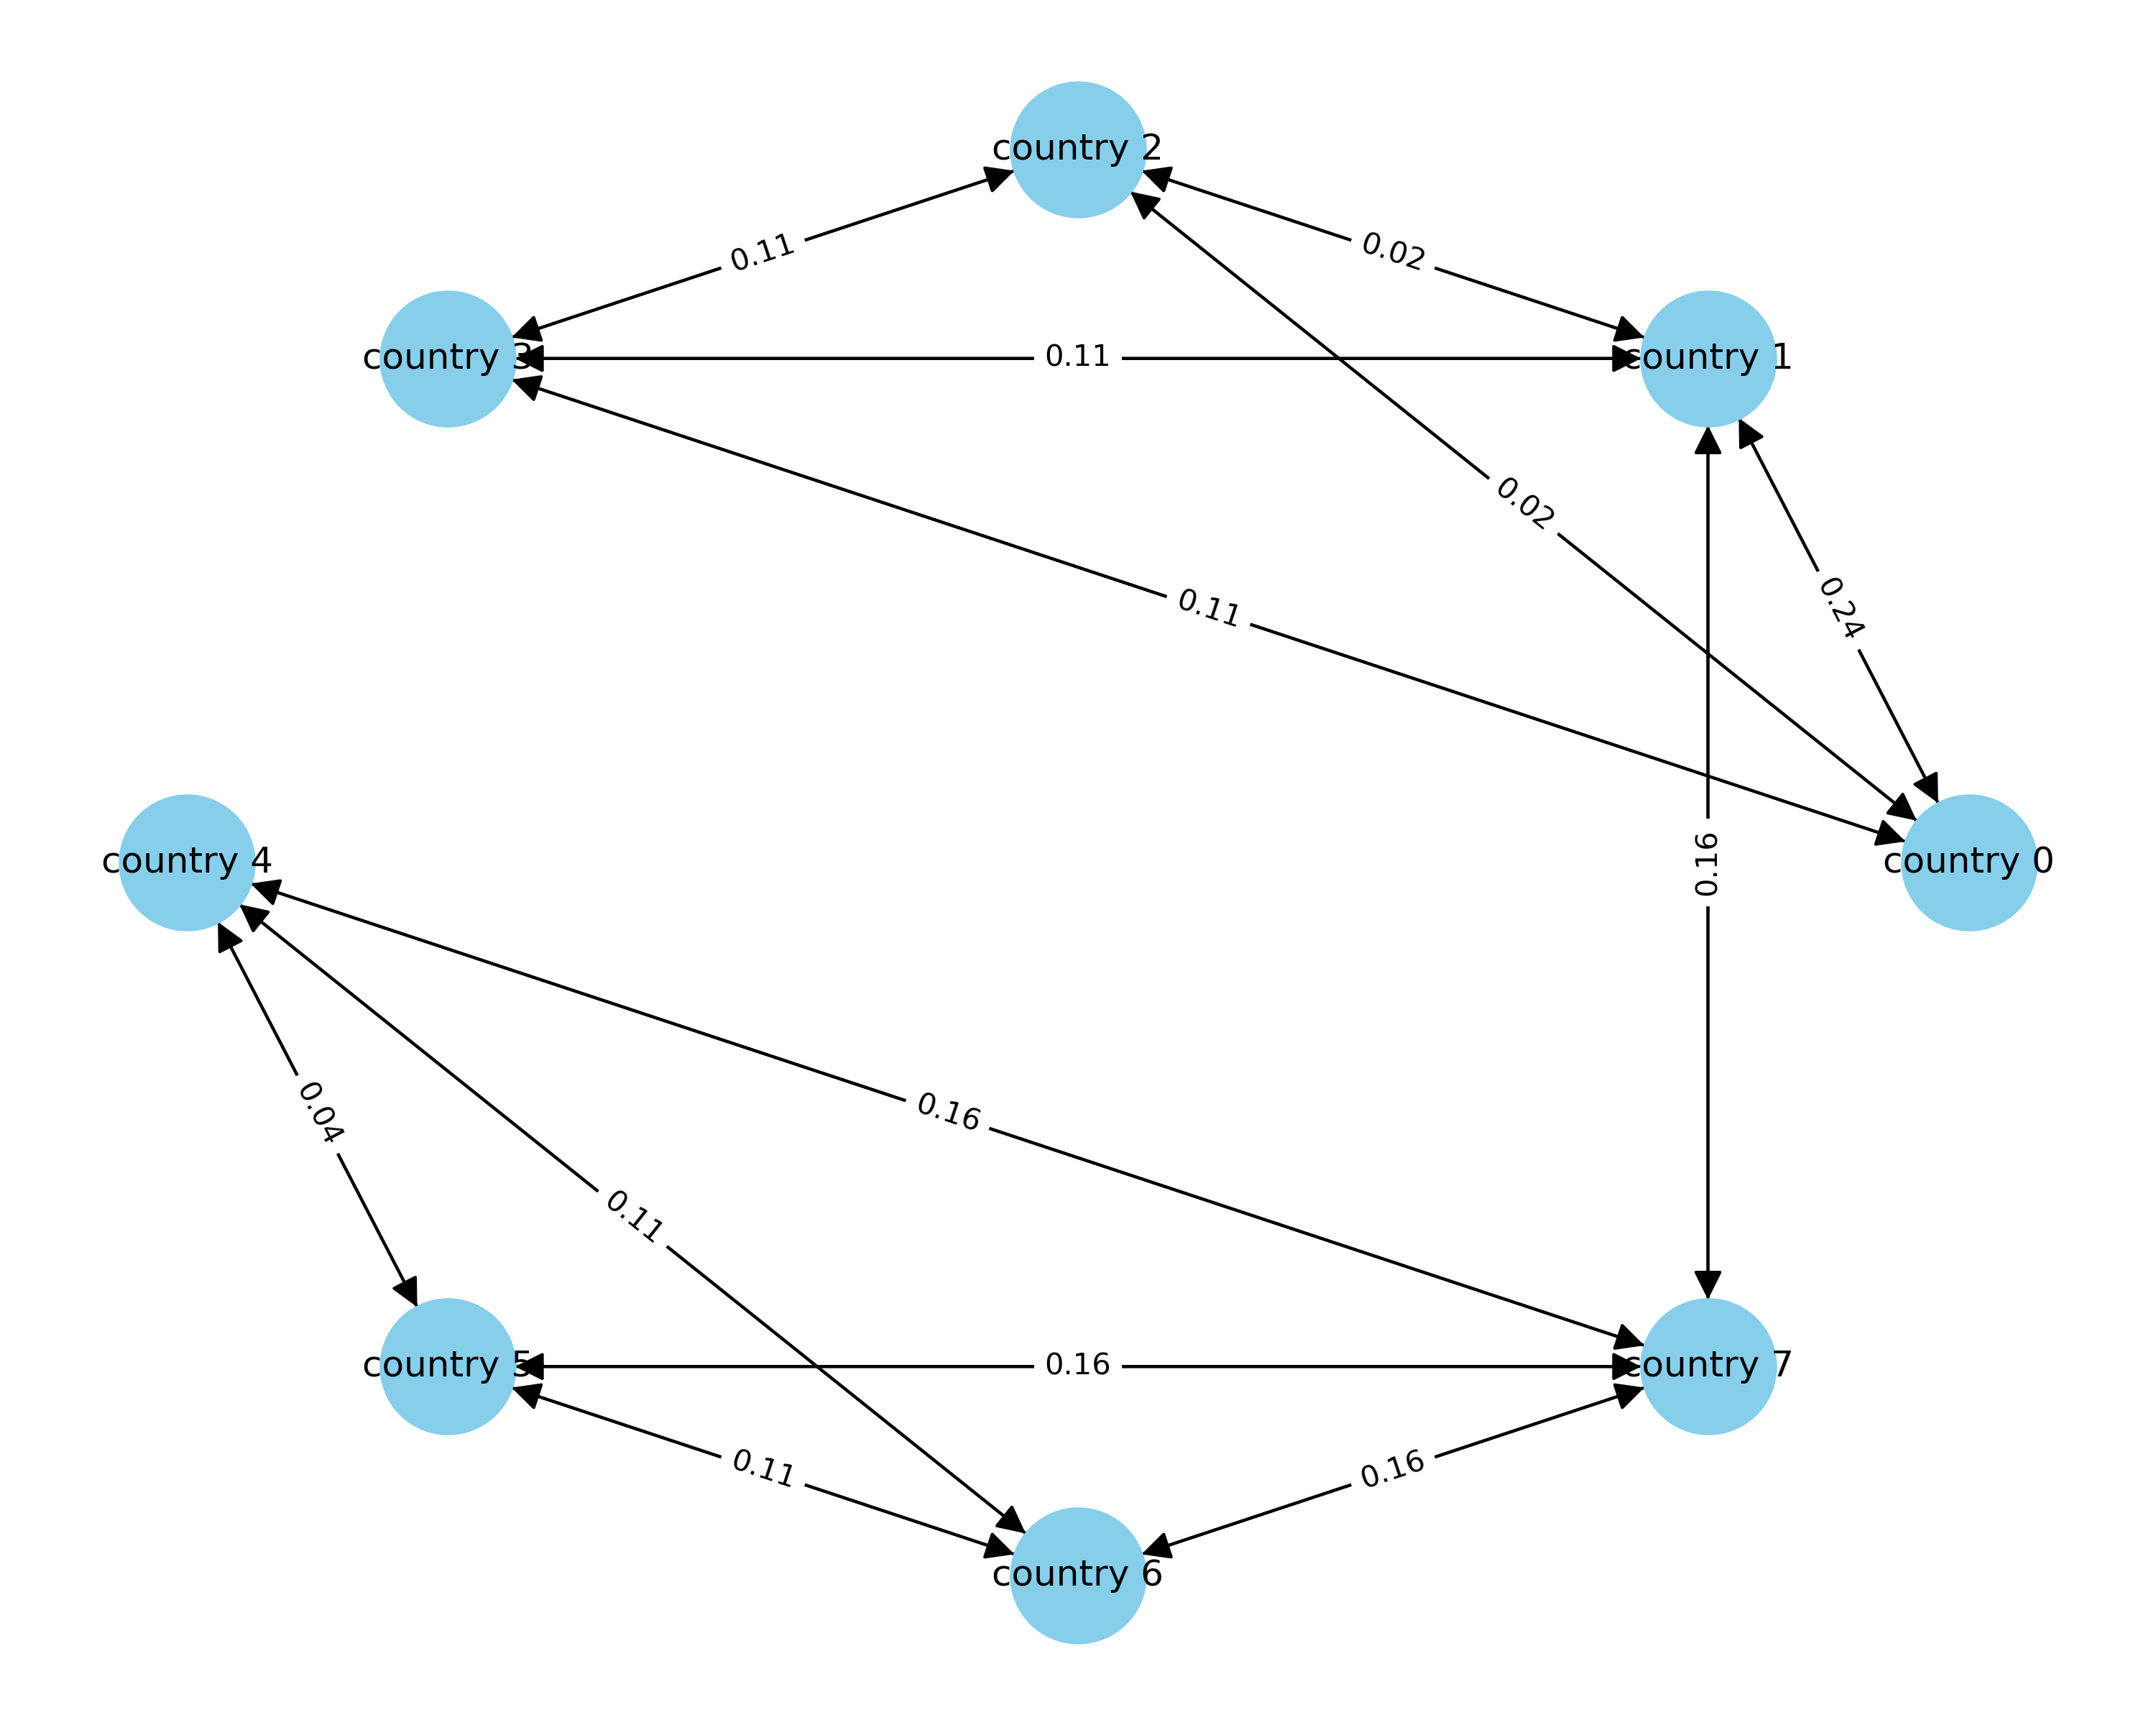
\includegraphics[width=0.8\textwidth]{../directed_graph.png}
    \caption{network graph}
    \label{fig: directed_graph.png}
\end{figure}
\FloatBarrier
\newpage
We can then graph our GDP over time (350 years) after which we will see it converge towards ~65 trillion \$  
\begin{figure}[htbp]
    \centering
    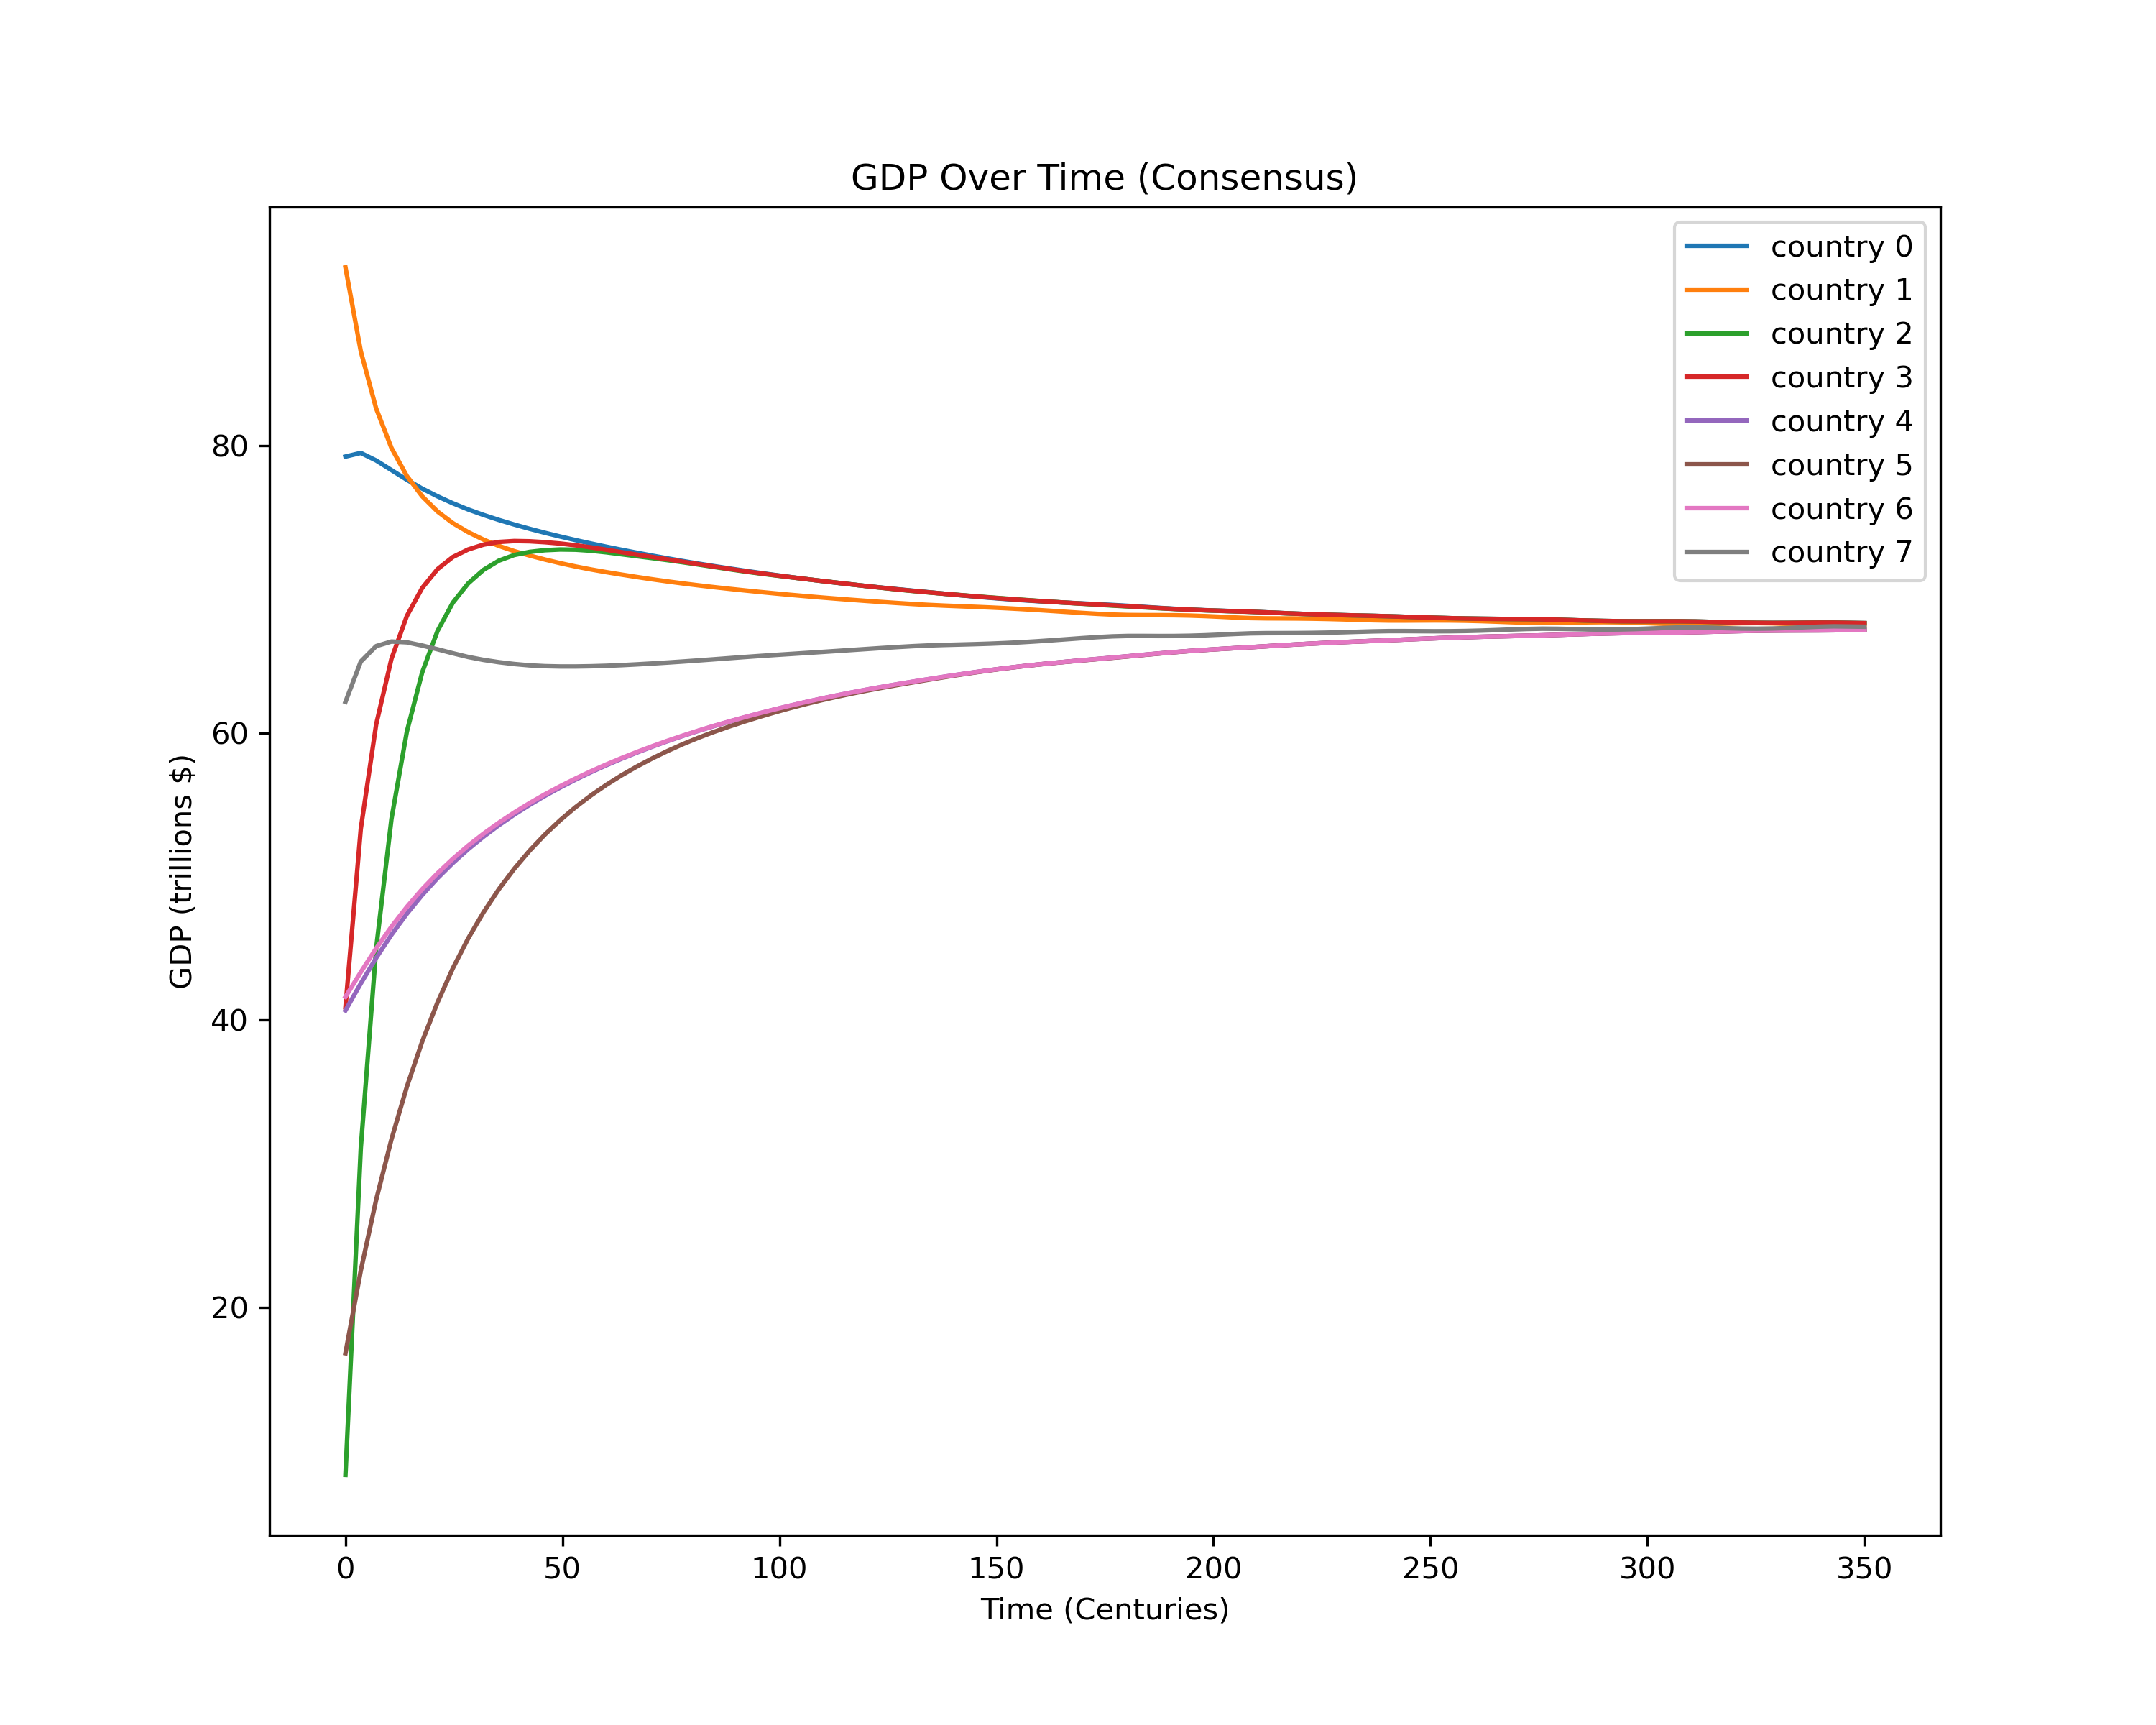
\includegraphics[width=0.8\textwidth]{../consensus.png}
    \caption{GDP vs Time}
    \label{fig: consensus.png}
\end{figure}
\FloatBarrier
we can see the stronger effects of higher GDP countries on lower GDP countries by observing how countries with a lower GDP improve their GDP rapidly whereas countries with a higher GDP change slower. The fact that we adjust the weights dynamically is only visible in the blue and grey lines where in the first 15 years they are sharply changing and later they slowly stabilize before trending towards convergence around 65 

\end{document}